\section{The Lattice of Subgroups of a Group}

\Exercise1 Let $H$ and $K$ be subgroups of $G$. Exhibit all possible
sublattices which show only $G$, $1$, $H$, $K$ and their joins and
intersections. What distinguishes the different drawings?
\begin{solution}
  In general, when $H$ and $K$ are distinct, with a nontrivial
  intersection and a join that is a proper subgroup, the sublattice
  might look something like the following:
  \begin{center}
    \begin{tikzpicture}
      \node at (0,3.5) {};
      \node (G) at (0,3) {$G$};
      \node (join) at (0,2) {$\gen{H,K}$};
      \node (H) at (-1,1) {$H$};
      \node (K) at (1,1) {$K$};
      \node (cap) at (0,0) {$H\cap K$};
      \node (1) at (0,-1) {$1$};
      \node at (0,-1.5) {};
      \draw (G) -- (join) -- (H) -- (cap) -- (K) -- (join);
      \draw (cap) -- (1);
    \end{tikzpicture}
  \end{center}
  In other cases, we may have $H = K$, or $H\geq K$:
  \begin{center}
    \begin{tikzpicture}
      \begin{scope}[xshift=-1.5cm]
        \node at (0,3.5) {};
        \node (G) at (0,3) {$G$};
        \node (HK) at (0,1.5){$H = K$};
        \node (1) at (0,0) {$1$};
        \node at (0,-0.5) {};
        \draw (G) -- (HK) -- (1);
      \end{scope}
      \begin{scope}[xshift=1.5cm]
        \node at (0,3.5) {};
        \node (G) at (0,3) {$G$};
        \node (H) at (0,2) {$H$};
        \node (K) at (0,1) {$K$};
        \node (1) at (0,0) {$1$};
        \node at (0,-0.5) {};
        \draw (G) -- (H) -- (K) -- (1);
      \end{scope}
    \end{tikzpicture}
  \end{center}
  There are several other possibilities, for example one of $H$ or $K$
  could be trivial, or we could have $\gen{H,K} = G$, and various
  other options. The drawings are distinguished by the relationships
  between the various subgroups.
\end{solution}

\Exercise2 In each of (a) to (d) list all subgroups of $D_{16}$ that
satisfy the given condition.
\begin{enumerate}
\item Subgroups that are contained in $\gen{sr^2,r^4}$
  \begin{solution}
    From the lattice given in the text, we see that the subgroups
    contained in $\gen{sr^2,r^4}$ are $\gen{sr^2,r^4}$, $\gen{sr^6}$,
    $\gen{sr^2}$, $\gen{r^4}$, and $1$.
  \end{solution}
\item Subgroups that are contained in $\gen{sr^7, r^4}$
  \begin{solution}
    $\gen{sr^7, r^4} = \gen{sr^3, r^4}$, so the subgroups contained in
    this subgroup are $\gen{sr^3, r^4}$, $\gen{r^4}$, $\gen{sr^3}$,
    $\gen{sr^7}$, and $1$.
  \end{solution}
\item Subgroups that contain $\gen{r^4}$
  \begin{solution}
    The subgroups containing $\gen{r^4}$ are $\gen{r^4}$,
    $\gen{sr^2,r^4}$, $\gen{s,r^4}$, $\gen{r^2}$, $\gen{sr^3,r^4}$,
    $\gen{sr^5,r^4}$, $\gen{s, r^2}$, $\gen{r}$, $\gen{sr, r^2}$, and
    $D_{16}$ itself.
  \end{solution}
\item Subgroups that contain $\gen{s}$
  \begin{solution}
    The subgroups containing $\gen{s}$ are $\gen{s}$, $\gen{s,r^4}$,
    $\gen{s,r^2}$, and $D_{16}$.
  \end{solution}
\end{enumerate}

\Exercise3 Show that the subgroup $\gen{s, r^2}$ of $D_8$ is
isomorphic to $V_4$.
\begin{proof}
  The subgroup $\gen{s, r^2}$ consists of the elements
  $\{1, s, r^2, sr^2\}$, and $V_4 = \{1, a, b, c\}$. Note that both
  groups are abelian and of order $4$.

  Define the mapping $\varphi\colon\gen{s,r^2}\to V_4$ by
  \begin{equation*}
    \varphi(1) = 1,
    \quad
    \varphi(s) = a,
    \quad
    \varphi(r^2) = b,
    \quad\text{and}\quad
    \varphi(sr^2) = c.
  \end{equation*}
  We now directly verify that $\varphi$ is a homomorphism:
  \begin{align*}
    \varphi(s^2) &= \varphi(1) = 1 = a^2 = \varphi(s)^2, \\
    \varphi(sr^2) &= c = ab = \varphi(s)\varphi(r^2), \\
    \varphi(ssr^2) &= \varphi(r^2) = b = ac = \varphi(s)\varphi(sr^2), \\
    \varphi(r^4) &= \varphi(1) = 1 = b^2 = \varphi(r^2)^2, \\
    \varphi(r^2sr^2) &= \varphi(s) = a = bc = \varphi(r^2)\varphi(sr^2), \\
    \varphi((sr^2)^2) &= \varphi(1) = 1 = c^2 = \varphi(sr^2)^2.
  \end{align*}
  Since both groups are abelian, this is enough to show that $\varphi$
  is a homomorphism. But $\varphi$ is clearly also a bijection, so
  $\varphi$ is an isomorphism and $\gen{s,r^2}\cong V_4$.
\end{proof}

\Exercise4 Use the given lattice to find all pairs of elements that
generate $D_8$ (there are $12$ pairs).
\begin{solution}
  First, we know that $D_8 = \gen{s,r}$. Now, looking at the cyclic
  subgroups in the lattice, we see that the only subgroup containing
  both $\gen{s}$ and $\gen{rs}$ is $D_8$ itself. Hence
  $\gen{s, rs} = D_8$. Similarly, the only subgroup containing
  $\gen{s}$ and $\gen{r^3s}$ is $D_8$, so $\gen{s, r^3s} =
  D_8$. Continuing in this way, we can find all the pairs that
  generate $D_8$ (noting that $\gen{r} = \gen{r^3}$):
  \begin{multline*}
    \gen{s,r}, \gen{s,r^3}, \gen{s,rs}, \gen{s,r^3s},
    \gen{r^2s,r}, \gen{r^2s,r^3}, \\
    \gen{r^2s,rs}, \gen{r^2s,r^3s},
    \gen{r,rs}, \gen{r^3,rs}, \gen{r^3,r^3s}, \gen{r,r^3s}.
  \end{multline*}
  No other pairing can generate all of $D_8$.
\end{solution}

\Exercise5 Use the given lattice to find all elements $x\in D_{16}$
such that $D_{16} = \gen{x, s}$ (there are $8$ such elements $x$).
\begin{solution}
  Note that $\gen{r} = \gen{r^3} = \gen{r^5} = \gen{r^7}$. We now
  proceed as in the previous problem, pairing $\gen{s}$ with other
  cyclic subgroups such that all of $D_{16}$ is the smallest group
  containing both subgroups. We find the following generating pairs:
  \begin{equation*}
    \gen{s,r},\gen{s,r^3},\gen{s,r^5},\gen{s,r^7},
    \gen{s,sr^3}, \gen{s,sr^7},\gen{s,sr^5},\gen{s,sr}.
    \qedhere
  \end{equation*}
\end{solution}

\Exercise6 Use the given lattices to help find the centralizers of
every element in the following groups:
\begin{enumerate}
\item $D_8$
  \begin{solution}
    Since $s$ commutes with $r^2$, we see from the lattice that
    $C_{D_8}(s) = \gen{s, r^2}$ (this centralizer cannot be all of
    $D_8$ since $s$ does not commute with $r$). $r^2$ commutes with
    everything (it is in the center of $D_8$), so
    $C_{D_8}(r^2) = D_8$. By similar reasoning, we find the following
    centralizers:
    \begin{align*}
      C_{D_8}(1) &= D_8, \\
      C_{D_8}(r) &= \gen{r}, \\
      C_{D_8}(r^2) &= D_8, \\
      C_{D_8}(r^3) &= \gen{r}, \\
      C_{D_8}(s) &= \gen{s, r^2}, \\
      C_{D_8}(rs) &= \gen{rs,r^2}, \\
      C_{D_8}(r^2s) &= \gen{s, r^2}, \\
      C_{D_8}(r^3s) &= \gen{rs, r^2}. \qedhere
    \end{align*}
  \end{solution}
\item $Q_8$
  \begin{solution}
    We know that $-1$ commutes with every element, but $i$, $j$, and
    $k$ do not commute with each other. Therefore
    \begin{align*}
      C_{Q_8}(1) &= Q_8, \\
      C_{Q_8}(-1) &= Q_8, \\
      C_{Q_8}(i) = C_{Q_8}(-i) &= \gen{i}, \\
      C_{Q_8}(j) = C_{Q_8}(-j) &= \gen{j}, \\
      C_{Q_8}(k) = C_{Q_8}(-k) &= \gen{k}. \qedhere
    \end{align*}
  \end{solution}
\item $S_3$
  \begin{solution}
    From the lattice we see that every nontrivial subgroup is maximal,
    so the centralizer of each cycle is either the subgroup generated
    by that cycle, or else all of $S_3$. But none of $(1\,2)$,
    $(1\,3)$, $(2\,3)$, and $(1\,2\,3)$ commute with each other, so
    none of the centralizers can be all of $S_3$, aside from
    $C_{S_3}(1)$. This gives
    \begin{align*}
      C_{S_3}(1) &= S_3, \\
      C_{S_3}(1\,2) &= \gen{(1\,2)}, \\
      C_{S_3}(1\,3) &= \gen{(1\,3)}, \\
      C_{S_3}(2\,3) &= \gen{(2\,3)}, \\
      C_{S_3}(1\,2\,3) = C_{S_3}(1\,3\,2) &= \gen{(1\,2\,3)}. \qedhere
    \end{align*}
  \end{solution}
\item $D_{16}$
  \begin{solution}
    We use similar reasoning as we did for $D_8$.
    \begin{align*}
      C_{D_{16}}(1) &= D_{16}, \\
      C_{D_{16}}(r) = C_{D_{16}}(r^2) = C_{D_{16}}(r^3) &= \gen{r}, \\
      C_{D_{16}}(r^5) = C_{D_{16}}(r^6) = C_{D_{16}}(r^7) &= \gen{r}, \\
      C_{D_{16}}(r^4) &= D_{16}, \\
      C_{D_{16}}(s) = C_{D_{16}}(sr^4) &= \gen{s, r^4}, \\
      C_{D_{16}}(sr) = C_{D_{16}}(sr^5) &= \gen{sr^5, r^4}, \\
      C_{D_{16}}(sr^2) = C_{D_{16}}(sr^6) &= \gen{sr^2, r^4}, \\
      C_{D_{16}}(sr^3) = C_{D_{16}}(sr^7) &= \gen{sr^3, r^4}. \qedhere
    \end{align*}
  \end{solution}
\end{enumerate}

\Exercise7 Find the center of $D_{16}$.
\begin{solution}
  We already found in Exercise~\ref{exercise:center-of-D2n} that
  $Z(D_{2n}) = 1$ if $n$ is odd and $Z(D_{2n}) = \{1, r^k\}$ if
  $n = 2k$. Therefore $Z(D_{16}) = \{1, r^4\}$. Alternatively, we
  could use the results from the previous problem, where we saw that
  $1$ and $r^4$ were the only elements with centralizers equal to all
  of $D_{16}$.
\end{solution}

\Exercise8 In each of the following groups find the normalizer of each
subgroup:
\begin{enumerate}
\item $S_3$
  \begin{solution}
    $S_3$ has six subgroups. From the lattice, we see that each
    nontrivial proper subgroup $H$ of $S_3$ is maximal, so we either
    have $N_{S_3}(H) = H$ or $N_{S_3}(H) = S_3$.

    For $H = \gen{(1\,2)}$, since
    \begin{equation*}
      (1\,3)(1\,2)(1\,3) = (2\,3) \not\in \gen{(1\,2)},
    \end{equation*}
    we see that $(1\,3)H(1\,3)^{-1} \neq H$, so $N_{S_3}(H) = H$. The
    same is true for the other subgroups generated by $2$-cycles. So,
    \begin{multline*}
      N_{S_3}(\gen{(1\,2)}) = \gen{(1\,2)},
      \quad
      N_{S_3}(\gen{(1\,3)}) = \gen{(1\,3)}, \\
      \text{and}\quad
      N_{S_3}(\gen{(2\,3)}) = \gen{(2\,3)}.
    \end{multline*}
    For $H = \gen{(1\,2\,3)} = \{1,(1\,2\,3),(1\,3\,2)\}$, we have
    \begin{align*}
      (1\,2)(1\,2\,3)(1\,2) &= (1\,3\,2)\in H, \\
      (1\,2)(1\,3\,2)(1\,2) &= (1\,2\,3)\in H,
    \end{align*}
    so $(1\,2)$ is in the normalizer of $H$. Therefore
    \begin{equation*}
      N_{S_3}(\gen{1\,2\,3}) = N_{S_3}(1) = N_{S_3}(S_3) = S_3. \qedhere
    \end{equation*}
  \end{solution}
\item $Q_8$
  \begin{solution}
    Since $1$ and $-1$ are in the center of $Q_8$, we have
    \begin{equation*}
      N_{Q_8}(1) = N_{Q_8}(-1) = N_{Q_8}(Q_8) = Q_8.
    \end{equation*}
    The other subgroups are maximal, so each normalizer is either the
    subgroup itself or else all of $Q_8$. Since
    \begin{align*}
      j(i)j^{-1} &= (-k)(-j) = kj = -i\in\gen{i}, \\ \intertext{and}
      j(-i)j^{-1} &= k(-j) = -kj = i\in\gen{i},
    \end{align*}
    we see that $j\in N_{Q_8}(\gen{i})$. Therefore
    $N_{Q_8}(\gen{i}) = Q_8$. By an entirely similar argument, we see
    that the same is true for $\gen{j}$ and $\gen{k}$. So
    \begin{equation*}
      N_{Q_8}(\gen{i}) = N_{Q_8}(\gen{j}) = N_{Q_8}(\gen{k}) = Q_8. \qedhere
    \end{equation*}
  \end{solution}
\end{enumerate}

\Exercise9 Draw the lattices of subgroups of the following groups:
\begin{enumerate}
\item $\Z/16\Z$
  \begin{solution}\;
      \begin{center}
        \begin{tikzpicture}
          \node (16) at (0,0) {$\gen{16} = \gen0$};
          \node (8) at (0,1) {$\gen{8}$};
          \node (4) at (0,2) {$\gen{4}$};
          \node (2) at (0,3) {$\gen{2}$};
          \node (1) at (0,4) {$\Z/16\Z$};
          \draw (16) -- (8) -- (4) -- (2) -- (1);
        \end{tikzpicture}
      \end{center}
  \end{solution}
\item $\Z/24\Z$
  \begin{solution}\;
    \begin{center}
      \begin{tikzpicture}
        \node (24) at (0,0) {$\gen{24} = \gen0$};
        \node (12) at (1,1) {$\gen{12}$};
        \node (8) at (-1,1.5) {$\gen{8}$};
        \node (6) at (2,2) {$\gen{6}$};
        \node (4) at (0,2.5) {$\gen{4}$};
        \node (3) at (3,3) {$\gen{3}$};
        \node (2) at (1,3.5) {$\gen{2}$};
        \node (1) at (2,4.5) {$\Z/24\Z$};
        \draw (24) -- (12) -- (6) -- (3) -- (1);
        \draw (24) -- (8) -- (4) -- (2) -- (1);
        \draw (12) -- (4);
        \draw (6) -- (2);
      \end{tikzpicture}
    \end{center}
  \end{solution}
\item $\Z/48\Z$
  \begin{solution}\;
    \begin{center}
      \begin{tikzpicture}
        \node (48) at (0,0) {$\gen{48} = \gen0$};
        \node (24) at (1,1) {$\gen{24}$};
        \node (16) at (-1,1.5) {$\gen{16}$};
        \node (12) at (2,2) {$\gen{12}$};
        \node (8) at (0,2.5) {$\gen{8}$};
        \node (6) at (3,3) {$\gen{6}$};
        \node (4) at (1,3.5) {$\gen{4}$};
        \node (3) at (4,4) {$\gen{3}$};
        \node (2) at (2,4.5) {$\gen{2}$};
        \node (1) at (3,5.5) {$\Z/48\Z$};
        \draw (48) -- (24) -- (12) -- (6) -- (3) -- (1);
        \draw (48) -- (16) -- (8) -- (4) -- (2) -- (1);
        \draw (24) -- (8);
        \draw (12) -- (4);
        \draw (6) -- (2);
      \end{tikzpicture}
    \end{center}
  \end{solution}
\end{enumerate}

\Exercise{10} Classify groups of order $4$ by proving that if
$\ord{G} = 4$ then $G\cong Z_4$ or $G\cong V_4$.
\label{exercise:classify:groups-4}
\begin{proof}
  Let $G = \{1,a,b,c\}$. If $G$ is cyclic, then certainly $G\cong Z_4$
  since all cyclic groups of the same order are isomorphic. So assume
  that $G$ is not cyclic, so that no element has order $4$. Since the
  order of each element must divide the order of the group, it follows
  that $a$, $b$, $c$ each have order $2$.

  Now consider the product $ab$. If $ab = 1$, then multiplying by $a$
  on the left gives $b = a$, so $a$ and $b$ are not distinct, which is
  a contradiction. If $ab = a$, then multiplying by $a$ gives $b = 1$,
  another contradiction. For the same reason we cannot have $ab =
  b$. So the only possibility is $ab = c$.

  Using exactly the same argument, we can see that $ba = c$,
  $ac = ca = b$, and $bc = cb = a$. Since $G$ has the same
  multiplication table as $V_4$, it follows that $G\cong V_4$. Indeed,
  any identity-preserving bijection between them is an isomorphism.
\end{proof}

\Exercise{11} Consider the group of order $16$ with the following
presentation:
\begin{equation*}
  QD_{16} = \gen{\sigma,\tau \mid \sigma^8 = \tau^2 = 1,\;
    \sigma\tau = \tau\sigma^3}
\end{equation*}
(called the {\em quasidihedral} or {\em semidihedral} group of order
$16$). This group has three subgroups of order $8$:
$\gen{\tau,\sigma^2}\cong D_8$, $\gen{\sigma} \cong Z_8$ and
$\gen{\sigma^2,\sigma\tau}\cong Q_8$ and every proper subgroup is
contained in one of these three subgroups. Fill in the missing
subgroups in the provided lattice of all subgroups of the
quasidihedral group, exhibiting each subgroup with at most two
generators.
\label{exercise:lattice:QD16}
\begin{solution}
  Certainly $\gen{\sigma^2}$ is between $\gen{\sigma}$ and
  $\gen{\sigma^4}$. By taking powers of the other elements, we see
  that the other missing cyclic subgroups are
  \begin{align*}
    \gen{\tau\sigma} &= \{1, \tau\sigma, \sigma^4, \tau\sigma^5\}, \\
    \gen{\tau\sigma^3} &= \{1, \tau\sigma^3, \sigma^4, \tau\sigma^7\}, \\
    \gen{\tau\sigma^4} &= \{1, \tau\sigma^4\}. \\\intertext{and}
    \gen{\tau\sigma^6} &= \{1, \tau\sigma^6\}.
  \end{align*}
  $\gen{\sigma^4,\tau}$ must contain $\gen{\tau\sigma^4}$, and we see
  that $\gen{\tau\sigma^6}$ must be the sibling of
  $\gen{\tau\sigma^2}$, whose containing subgroup would then be
  $\gen{\sigma^4, \tau\sigma^2}$. The remaining cyclic subgroups are
  contained in $\gen{\sigma^2, \tau\sigma}$. This gives the following
  lattice.
  \begin{center}
    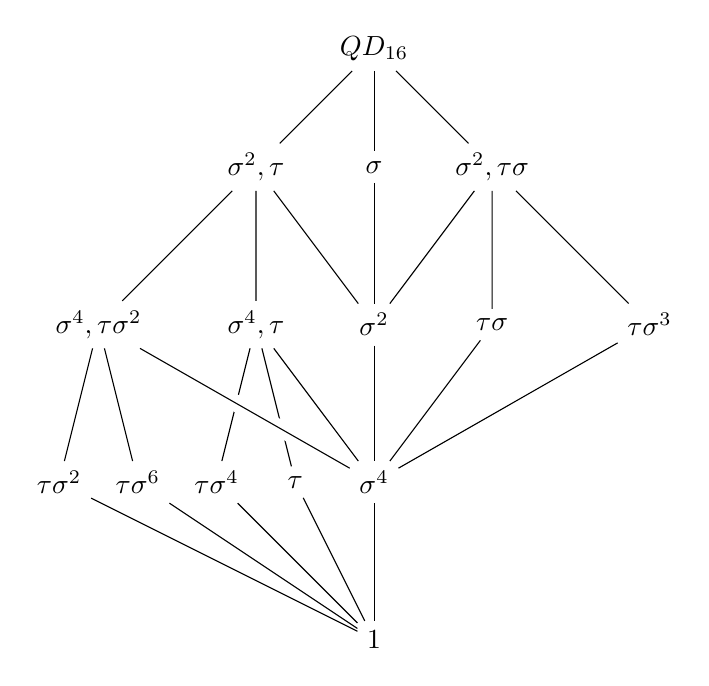
\begin{tikzpicture}
      \node (1) at (0,0) {$1$};
      \node (sigma4) at (0,2) {$\gen{\sigma^4}$};
      \node (tau) at (-1,2) {$\gen{\tau}$};
      \node (tausigma4) at (-2,2) {$\gen{\tau\sigma^4}$};
      \node (tausigma6) at (-3,2) {$\gen{\tau\sigma^6}$};
      \node (tausigma2) at (-4,2) {$\gen{\tau\sigma^2}$};
      \node (sigma2) at (0,4) {$\gen{\sigma^2}$};
      \node (sigma4_tau) at (-1.5,4) {$\gen{\sigma^4,\tau}$};
      \node (sigma4_tausigma2) at (-3.5,4) {$\gen{\sigma^4,\tau\sigma^2}$};
      \node (tausigma) at (1.5,4) {$\gen{\tau\sigma}$};
      \node (tausigma3) at (3.5,4) {$\gen{\tau\sigma^3}$};
      \node (sigma) at (0,6) {$\gen{\sigma}$};
      \node (sigma2_tau) at (-1.5,6) {$\gen{\sigma^2,\tau}$};
      \node (sigma2_tausigma) at (1.5,6) {$\gen{\sigma^2,\tau\sigma}$};
      \node (QD16) at (0,7.5) {$QD_{16}$};
      \draw (QD16) -- (sigma) -- (sigma2) -- (sigma4) -- (1);
      \draw (QD16) -- (sigma2_tau) -- (sigma4_tau) -- (tau) -- (1);
      \draw (QD16) -- (sigma2_tausigma) -- (tausigma) -- (sigma4);
      \draw (sigma2_tau) -- (sigma4_tausigma2) -- (tausigma6) -- (1);
      \draw (sigma2_tau) -- (sigma2) -- (sigma2_tausigma);
      \draw (sigma2_tausigma) -- (tausigma3) -- (sigma4);
      \draw (sigma4_tau) -- (sigma4);
      \draw (sigma4_tau) -- (tausigma4) -- (1);
      \draw (sigma4_tausigma2) -- (tausigma2) -- (1);
      \draw[draw=white,line width=6pt] (sigma4_tausigma2) -- (sigma4);
      \draw (sigma4_tausigma2) -- (sigma4);
    \end{tikzpicture}
  \end{center}
\end{solution}

\Exercise{12} The group
\begin{equation*}
  A = Z_2\times Z_4 = \gen{a,b\mid a^2 = b^4 = 1,\; ab = ba}
\end{equation*}
has order $8$ and has three subgroups of order $4$:
$\gen{a,b^2}\cong V_4$, $\gen{b}\cong Z_4$ and $\gen{ab}\cong Z_4$ and
every proper subgroup is contained in one of these three. Draw the
lattice of all subgroups of $A$ giving each subgroup in terms of at
most two generators.
\label{exercise:lattice:Z2-times-Z4}
\begin{solution}
  Writing out the elements of $A$ (in terms of $a$ and $b$) gives
  \begin{equation*}
    A = \{1, a, b, b^2, b^3, ab, ab^2, ab^3\}.
  \end{equation*}
  There are three elements with order $2$, namely $a$, $b^2$, and
  $ab^2$. Since $\gen{a,b^2}\cong V_4$, we see that $\gen{a}$,
  $\gen{b^2}$, and $\gen{ab^2}$ must be directly contained in
  $\gen{a,b^2}$. From this and the other given information, we form
  the following lattice.
  \begin{center}
    \begin{tikzpicture}[scale=1.25]
      \node (A) at (0,0) {$A$};
      \node (b) at (2, -2) {$\gen{b}$};
      \node (a_b2) at (-2, -2) {$\gen{a, b^2}$};
      \node (ab) at (0, -2) {$\gen{ab}$};
      \node (b2) at (0, -4) {$\gen{b^2}$};
      \node (a) at (-4, -4) {$\gen{a}$};
      \node (ab2) at (-2, -4) {$\gen{ab^2}$};
      \node (1) at (-2, -6) {$1$};
      \draw (A) -- (a_b2) -- (a) -- (1);
      \draw (a_b2) -- (ab2) -- (1);
      \draw (a_b2) -- (b2);
      \draw (A) -- (b) -- (b2) -- (1);
      \draw (A) -- (ab) -- (b2);
    \end{tikzpicture}
  \end{center}
\end{solution}

\Exercise{13} The group
\begin{equation*}
  G = Z_2\times Z_8 = \gen{x,y\mid x^2 = y^8 = 1,\; xy = yx}
\end{equation*}
has order $16$ and has three subgroups of order $8$:
$\gen{x,y^2}\cong Z_2\times Z_4$, $\gen{y}\cong Z_8$ and
$\gen{xy}\cong Z_8$ and every proper subgroup is contained in one of
these three. Draw the lattice of all subgroups of $G$, giving each
subgroup in terms of at most two generators.
\begin{solution}
  Since $\gen{x,y^2}\cong Z_2\times Z_4$, we see that the lattice of
  $G$ contains the lattice from the previous exercise within its
  structure, with $a$ replaced by $x$ and $b$ replaced by
  $y^2$. Adding in the maximal subgroups $\gen{y}$ and $\gen{xy}$
  produces the following lattice.
  \begin{center}
    \begin{tikzpicture}
      \node (G) at (2, 2) {$G$};
      \node (xy) at (2, 0) {$\gen{xy}$};
      \node (y) at (4, 0) {$\gen{y}$};
      \node (x_y2) at (0,0) {$\gen{x,y^2}$};
      \node (y2) at (2, -2) {$\gen{y^2}$};
      \node (x_y4) at (-2, -2) {$\gen{x, y^4}$};
      \node (xy2) at (0, -2) {$\gen{xy^2}$};
      \node (y4) at (0, -4) {$\gen{y^4}$};
      \node (x) at (-4, -4) {$\gen{x}$};
      \node (xy4) at (-2, -4) {$\gen{xy^4}$};
      \node (1) at (-2, -6) {$1$};
      \draw (G) -- (x_y2) -- (x_y4) -- (x) -- (1);
      \draw (G) -- (y) -- (y2) -- (y4) -- (1);
      \draw (G) -- (xy) -- (y2) -- (x_y2) -- (xy2) -- (y4)
      -- (x_y4) -- (xy4) -- (1);
    \end{tikzpicture}
  \end{center}
\end{solution}

\Exercise{14} Let $M$ be the group of order $16$ with the following
presentation:
\begin{equation*}
  \gen{u,v \mid u^2 = v^8 = 1, \; vu = uv^5}
\end{equation*}
(sometimes called the {\em modular} group of order $16$). It has three
subgroups of order $8$: $\gen{u,v^2}$, $\gen{v}$ and $\gen{uv}$ and
every proper subgroup is contained in one of these three. Prove that
$\gen{u,v^2}\cong Z_2\times Z_4$, $\gen{v}\cong Z_8$ and
$\gen{uv}\cong Z_8$. Show that the lattice of subgroups of $M$ is the
same as the lattice of subgroups of $Z_2\times Z_8$ but that these two
groups are not isomorphic.
\label{exercise:lattice:modular16}
\begin{solution}
  We will use the presentation for $Z_2\times Z_4$ given in
  Exercise~\ref{exercise:lattice:Z2-times-Z4}. Since
  $u^2 = (v^2)^4 = 1$ and $u(v^2) = (v^2)u$, it follows that the
  mapping $\varphi\colon Z_2\times Z_4\to\gen{u,v^2}$ defined by
  \begin{equation*}
    \varphi(a) = u
    \quad\text{and}\quad
    \varphi(b) = v^2
  \end{equation*}
  extends to a homomorphism. $\varphi$ is surjective by construction
  and hence bijective since we know that both groups $Z_2\times Z_4$
  and $\gen{u,v^2}$ have order $8$. Therefore
  $\gen{u,v^2}\cong Z_2\times Z_4$.

  Since we know $\ord{\gen{v}} = \ord{\gen{uv}} = 8$, we automatically
  know that both subgroups are isomorphic to $Z_8$, since all cyclic
  groups of the same order are isomorphic. We see that the subgroups
  of $M$ share the same relationships as the subgroups of
  $Z_2\times Z_8$, so they have the same lattice, with $x$ replaced by
  $u$ and $y$ replaced by $v$:
  \begin{center}
    \begin{tikzpicture}
      \node (G) at (2, 2) {$M$};
      \node (xy) at (2, 0) {$\gen{uv}$};
      \node (y) at (4, 0) {$\gen{v}$};
      \node (x_y2) at (0,0) {$\gen{u,v^2}$};
      \node (y2) at (2, -2) {$\gen{v^2}$};
      \node (x_y4) at (-2, -2) {$\gen{u, v^4}$};
      \node (xy2) at (0, -2) {$\gen{uv^2}$};
      \node (y4) at (0, -4) {$\gen{v^4}$};
      \node (x) at (-4, -4) {$\gen{u}$};
      \node (xy4) at (-2, -4) {$\gen{uv^4}$};
      \node (1) at (-2, -6) {$1$};
      \draw (G) -- (x_y2) -- (x_y4) -- (x) -- (1);
      \draw (G) -- (y) -- (y2) -- (y4) -- (1);
      \draw (G) -- (xy) -- (y2) -- (x_y2) -- (xy2) -- (y4)
      -- (x_y4) -- (xy4) -- (1);
    \end{tikzpicture}
  \end{center}

  Finally, we note that, despite having the same lattice, $M$ is not
  isomorphic to $Z_2\times Z_8$ since the latter is abelian and $M$ is
  not ($uv \neq vu$).
\end{solution}

\Exercise{15} Describe the isomorphism type of each of the three
subgroups of $D_{16}$ of order $8$.
\begin{solution}
  Since $\ord{r} = 8$, we see that $\gen{r}\cong Z_8$.

  Next, consider the subgroup $H = \gen{s,r^2}$ and observe that
  \begin{equation*}
    (r^2)^4 = s^2 = 1
    \quad\text{and}\quad
    (r^2)s = sr^6 = s(r^2)^{-1}.
  \end{equation*}
  Since $s$ and $r^2$ in $D_{16}$ satisfy the same relations as $s$
  and $r$ do in $D_8$, the map $\varphi\colon D_8\to H$ given by
  \begin{equation*}
    \varphi(r) = r^2
    \quad\text{and}\quad
    \varphi(s) = s
  \end{equation*}
  extends to a surjective homomorphism. And it is easy to see that $H$
  consists of only eight elements, namely elements of the form
  $s^ir^{2j}$ where $i\in\{0,1\}$ and $j\in\{0,1,2,3\}$. Therefore
  $\varphi$ must be a bijection, and we have $\gen{s,r^2}\cong D_8$.

  Now consider the subgroup $K = \gen{sr,r^2}$. We have
  \begin{equation*}
    (r^2)^4 = (sr)^2 = 1
    \quad\text{and}\quad
    (r^2)(sr) = sr^7 = (sr)(r^2)^{-1}.
  \end{equation*}
  So the map $\psi\colon D_8\to K$ given by
  \begin{equation*}
    \varphi(r) = r^2
    \quad\text{and}\quad
    \varphi(s) = sr
  \end{equation*}
  extends to a surjective homomorphism, which must be injective as
  well since $K$ has $8$ elements. Therefore $\gen{sr,r^2}\cong D_8$.
\end{solution}

\Exercise{16} Use the lattice of subgroups of the quasidihedral group
of order $16$ to show that every element of order $2$ is contained in
the proper subgroup $\gen{\tau,\sigma^2}$.
\begin{proof}
  Every element of order $2$ generates a cyclic subgroup having order
  $2$. From the lattice of $QD_{16}$
  (Exercise~\ref{exercise:lattice:QD16}) we see that every cyclic
  subgroup of $QD_{16}$ is contained in $\gen{\sigma^2,\tau}$ except
  for $\gen{\tau\sigma}$ and $\gen{\tau\sigma^3}$. But neither
  $\tau\sigma$ nor $\tau\sigma^3$ has order $2$ (they both have order
  $4$), so we see that every element of order $2$ is indeed contained
  in $\gen{\sigma^2,\tau}$.
\end{proof}

\Exercise{17} Use the lattice of subgroups of the modular group $M$ of
order $16$ to show that the set $\{x\in M\mid x^2 = 1\}$ is a subgroup
of $M$ isomorphic to the Klein $4$-group.
\begin{proof}
  We know from Exercise~\ref{exercise:classify:groups-4} that every
  group of order $4$ is isomorphic to either $Z_4$ or $V_4$. From the
  lattice we constructed in Exercise~\ref{exercise:lattice:modular16},
  we see that $\gen{u,v^4}$ contains only the four elements $1$, $u$,
  $v^4$, and $uv^4$. Since each of these (aside from $1$) has order
  $2$, we know that $\gen{u,v^4}$ is not cyclic and so cannot be
  isomorphic to $Z_4$. Therefore $\gen{u,v^4}\cong V_4$.
\end{proof}

\Exercise{18} Use the lattice to help find the centralizer of every
element of $QD_{16}$.
\begin{solution}
  Since $\sigma^4\tau = \tau\sigma^{12} = \tau\sigma^4$, we see that
  $\sigma^4$ commutes with $\tau$ and hence belongs to the center of
  the group (since it commutes with each generator).

  From the lattice, we see that the centralizer of $\tau$ is either
  equal to $\gen{\sigma^4,\tau}$, or to $\gen{\sigma^2,\tau}$, or to
  all of $QD_{16}$. But we can rule out the latter two cases, since
  $\tau$ does not commute with $\sigma^2$:
  \begin{equation*}
    \sigma^2\tau = \tau\sigma^6.
  \end{equation*}
  A similar case can be made for the centralizer of $\tau\sigma^4$.

  For $\tau\sigma^2$ and $\tau\sigma^6$ we see that both commute with
  $\sigma^4$ and $\tau\sigma^2$, but neither commutes with $\sigma^2$,
  so their centralizer must be $\gen{\sigma^4,\tau\sigma^2}$.

  $\tau\sigma$ and $\tau\sigma^3$ do not commute with $\sigma^2$, so
  their respective centralizers are just the cyclic subgroups that
  they generate.

  Lastly, the powers of $\sigma$ all commute with each other. Putting
  all this information together, we get
  \begin{align*}
    C_{QD_{16}}(1) = C_{QD_{16}}(\sigma^4) &= QD_{16}, \\
    C_{QD_{16}}(\sigma) = C_{QD_{16}}(\sigma^2)
    = C_{QD_{16}}(\sigma^3) &= \gen{\sigma}, \\
    C_{QD_{16}}(\sigma^5) = C_{QD_{16}}(\sigma^6)
    = C_{QD_{16}}(\sigma^7) &= \gen{\sigma}, \\
    C_{QD_{16}}(\tau) = C_{QD_{16}}(\tau\sigma^4) &= \gen{\sigma^4,\tau}, \\
    C_{QD_{16}}(\tau\sigma^2)
    = C_{QD_{16}}(\tau\sigma^6) &= \gen{\sigma^4,\tau\sigma^2}, \\
    C_{QD_{16}}(\tau\sigma)
    = C_{QD_{16}}(\tau\sigma^5) &= \gen{\tau\sigma}, \\
    C_{QD_{16}}(\tau\sigma^3)
    = C_{QD_{16}}(\tau\sigma^7) &= \gen{\tau\sigma^3}. \qedhere
  \end{align*}
\end{solution}

\Exercise{19} Use the lattice to help find $N_{D_{16}}(\gen{s,r^4})$.
\begin{solution}
  Let $H = \gen{s,r^4}$. From the lattice, we see that the normalizer
  of $H$ must be either $H$ itself, or $\gen{s,r^2}$, or
  $D_{16}$. Since
  \begin{align*}
    r^2(r^4)(r^2)^{-1} = r^2r^4r^6 &= r^4\in H, \\
    r^2s(r^2)^{-1} = r^2sr^6 &= sr^4\in H, \\
    \intertext{and}
    r^2(sr^4)(r^2)^{-1} = r^2sr^2 &= s\in H,
  \end{align*}
  we see that $r^2H(r^2)^{-1} = H$ so $\gen{s,r^2}\leq
  N_{D_{16}}(H)$. However, since
  \begin{equation*}
    rsr^7 = sr^7r^7 = sr^6 \not\in H,
  \end{equation*}
  we see that $rHr^{-1}\neq H$ so the normalizer of $H$ cannot be all
  of $D_{16}$. Therefore $N_{D_{16}}(H) = \gen{s,r^2}$.
\end{solution}

\Exercise{20} Use the lattice of subgroups of $QD_{16}$ to help find
the normalizers
\begin{enumerate}
\item $N_{QD_{16}}(\gen{\tau\sigma})$
  \begin{solution}
    Let $H = \gen{\tau\sigma}$. From the lattice
    (Exercise~\ref{exercise:lattice:QD16}) we see that there are only
    three possibilities for the normalizer of $H$: it is either $H$
    itself, or $\gen{\sigma^2,\tau\sigma}$ or else all of
    $QD_{16}$. Since $H = \{1,\tau\sigma,\sigma^4,\tau\sigma^5\}$, we
    can compute the elements of $\sigma^2H(\sigma^2)^{-1}$ as follows:
    \begin{align*}
      \sigma^2(\tau\sigma)\sigma^6 = \tau\sigma^6\sigma^7
      &= \tau\sigma^5, \\
      \sigma^2\sigma^4\sigma^6 &= \sigma^4, \\
      \sigma^2(\tau\sigma^5)\sigma^6
      = \sigma^2\tau\sigma^3 &= \tau\sigma.
    \end{align*}
    So $\sigma^2H(\sigma^2)^{-1} = H$ and therefore $\sigma^2$ is in
    the normalizer of $H$. But $\sigma$ is not in the normalizer,
    since
    \begin{equation*}
      \sigma(\tau\sigma)\sigma^7 = \sigma\tau = \tau\sigma^3\not\in H.
    \end{equation*}
    Thus the only possibility is
    $N_{QD_{16}}(H) = \gen{\sigma^2,\tau\sigma}$.
  \end{solution}
\item $N_{QD_{16}}(\gen{\tau, \sigma^4})$
  \begin{solution}
    Let $K = \gen{\tau, \sigma^4}$. Again there are three
    possibilities. $K = \{1, \tau, \sigma^4, \tau\sigma^4\}$, so as
    before, we compute the elements of $\sigma^2K(\sigma^2)^{-1}$:
    \begin{align*}
      \sigma^2\tau\sigma^6 = \tau\sigma^{12} &= \tau\sigma^4, \\
      \sigma^2\sigma^4\sigma^6 &= \sigma^4, \\
      \sigma^2(\tau\sigma^4)\sigma^6 = \sigma^2\tau\sigma^2
      &= \tau.
    \end{align*}
    So $\sigma^2K(\sigma^2)^{-1} = K$ and we must have
    $\gen{\tau, \sigma^2}\leq N_{QD_{16}}(K)$. And since
    \begin{equation*}
      \sigma\tau\sigma^7 = \tau\sigma^2\not\in K,
    \end{equation*}
    we see that the normalizer cannot be all of $QD_{16}$. Therefore
    $N_{QD_{16}}(K) = \gen{\tau,\sigma^2}$.
  \end{solution}
\end{enumerate}
